
\documentclass[conference]{IEEEtran}
\usepackage{cite}
\usepackage{graphicx}
\usepackage{amsmath}
\usepackage{enumerate}
\usepackage{xcolor}
\usepackage{pgfplots}
\usepackage{tikz}

\definecolor{bblue}{HTML}{4F81BD}
\definecolor{rred}{HTML}{C0504D}
\definecolor{ggreen}{HTML}{9BBB59}
\definecolor{ppurple}{HTML}{9F4C7C}

% correct bad hyphenation here
\hyphenation{op-tical net-works semi-conduc-tor}


\begin{document}

\title{PRECINCT:\@ An Incremental Algorithm to Prevent Clone Insertion}


\author{\IEEEauthorblockN{Mathieu Nayrolles, }
\IEEEauthorblockA{Software Behaviour Analysis (SBA) Research Lab\\
ECE, Concordia University\\
Montreal, Canada\\
m\_nayrol@ece.concordia.ca}
\and
\IEEEauthorblockN{Abdelwahab Hamou-Lhadj}
\IEEEauthorblockA{Software Behaviour Analysis (SBA) Research Lab\\
ECE, Concordia University\\
Montreal, Canada\\
abdelw@ece.concordia.ca}}

% make the title area
\maketitle

% As a general rule, do not put math, special symbols or citations
% in the abstract
\begin{abstract}
  Software clones are considered harmful in software maintenance and evolution. However, after a decade and a half of research, only few approaches have targeted the prevention aspect of clones detection.
  In this paper, we propose a novel approach named PRECINCT (PREventing Clones INsertion at Commit Time). PRECINCT focuses on near-miss software clones are copied --- or reinvented --- fragments where minor to extensive modifications have been made and more specifically on detecting at commit time by means of pre-commit hooks.
  Efficiently detecting near-miss software clones at commit time might call for further refactoring or simply hint developers that they reinvented one piece of code.
  We apply and validate PRECINCT in terms of precision and recall on seven systems developed independently with a wide range of technologies, size and purposes.
  The validation demonstrates that our approach detects near-miss software clones before they reach the source version system with a 100\% precision and a 93\% recall.



\end{abstract}


\IEEEpeerreviewmaketitle

\section{Introduction}
\label{sec:Introduction}


Code or software clones appear when developers reuse code with little to no modification.
Previous research has shown that clones can account for 7\% to 50\% of a given software\cite{Baker, StephaneDucasse}.
Developers often reuse code and create clones in their software on purpose\cite{Kim2005}.
Nevertheless, clones are considered a bad practice in software development and therefore, harmful\cite{Kapser2006,Juergens2009,Li2006}.
The most obvious way a clone can hazardous for the quality of a software system is if a default or bug is discovered in one segment of code that has been copied pasted several times, then the developers would have to remember the places where this segment has been reused in order to fix the default in each of them.

In order to help developers to deal with clones, researchers and practitioners have published hundreds of studies and dozens of tools using different approaches:   (1) textual where the source code is considered as text and transformation or normalization is applied to it in order to compare it with order code fragment\cite{Johnson1994,Johnson1993, Cordy2011, Roy2008}.
(2) Lexical where the source code is sliced into sequences of tokens as a compiler would\cite{Baker,Bakera,Baker2002,Kamiya2002,Li2006}.
(3) Syntactic where the source code is converted into trees, more particularly abstract syntax tree (AST) and then, the clone detection is performed using tree matching algorithms\cite{Baxter1998, Komondoor2000, Tairas2006, Falke2008}.

Henceforth, clones detection can be considered as a mature and still active field of research with two decades of research and hundreds of publications.
Consequently, practitioners and engineers know that copy-pasting segment of code can hinder the maintenance and the quality of their systems and that approaches exist to detect them.
However, the use of such approaches and tools is not as widespread as one might think.
Indeed, as for automatic bug finding tools, the main reasons for this lack of infatuation are that these tools are known to have (1) massive outputs which is (2) hard to understand and contain (3) a high amount of false positives.
Moreover, these tools are (4) hard to configure and there is (5) little to no integration of these tools in the day-to-day workflow of a developer\cite{Johnson2013}.

In this paper, we present PRECINCT (PREventing Clones INsertion at Commit Time) that focuses on preventing the insertion of clones at commit time.
More specifically, our approach provides a clone detection process that eases the five major reasons that limit the adoption of such tools.
To do so, we use pre-commit hooks capabilities of modern source code version control.
A pre-commit hook is a process that one can implements to receive the latest modification to the source code done by a given developer just before the code reaches the central repository.
Then, analysis can be done using bash programming or calling external programs, allowing the changes to go through or not.
PRECINCT is, in fact, a pre-commit hook that detects clones that might have been inserted in the latest changes with regard to the rest of the source code.
Consequently, only a fraction of the code is analyzed and PRECINCTS reduce the output by 70\% (compared to the clone detector PRECINCTS is built upon NiCad\cite{Cordy2011}).
Moreover, the detected clones are presented in using a classical diff output that developers are used to.
Hence, concerns (1) \textit{massive outputs} and (2) \textit{hard to understand} are less than in other tools.
Also, PRECINCTS can be installed and configured using only one command line (\textit{hard to configure}).
Finally, our approach leverages the pre-commit hook capabilities of modern source code version control and therefore, integrates itself at the heart of the programmers workflow (\textit{little to no integration of these tools in the day-to-day workflow}).

We assessed the capabilities of PRECINCT in terms of precision and recall on seven systems developed independently with a wide range of technologies and purposes.
The validation demonstrates that our approach detects near-miss software clones before they reach the source version system with a 100\% precision and a 93\% recall while increasing the size of the repository by only 3\% to 5\%.

The rest of this paper is organized as follows: In Section~\ref{sec:Related Works} we present the works related to PRECINCT and with a particular attention of Nicad.
Then, in Section~\ref{sec:The PRECINCT Approach} we present the PRECINCT approach and Section~\ref{sec:Experimentations} shows the experimentations we conduct to assess the capacities of PRECINCT.
Finally, we propose some concluding remarks in Section~\ref{sec:Conclusion}.

\section{Related Works}
\label{sec:Related Works}



\section{The PRECINCT Approach}
\label{sec:The PRECINCT Approach}

In this section, we present the

\begin{figure*}
  \centering
    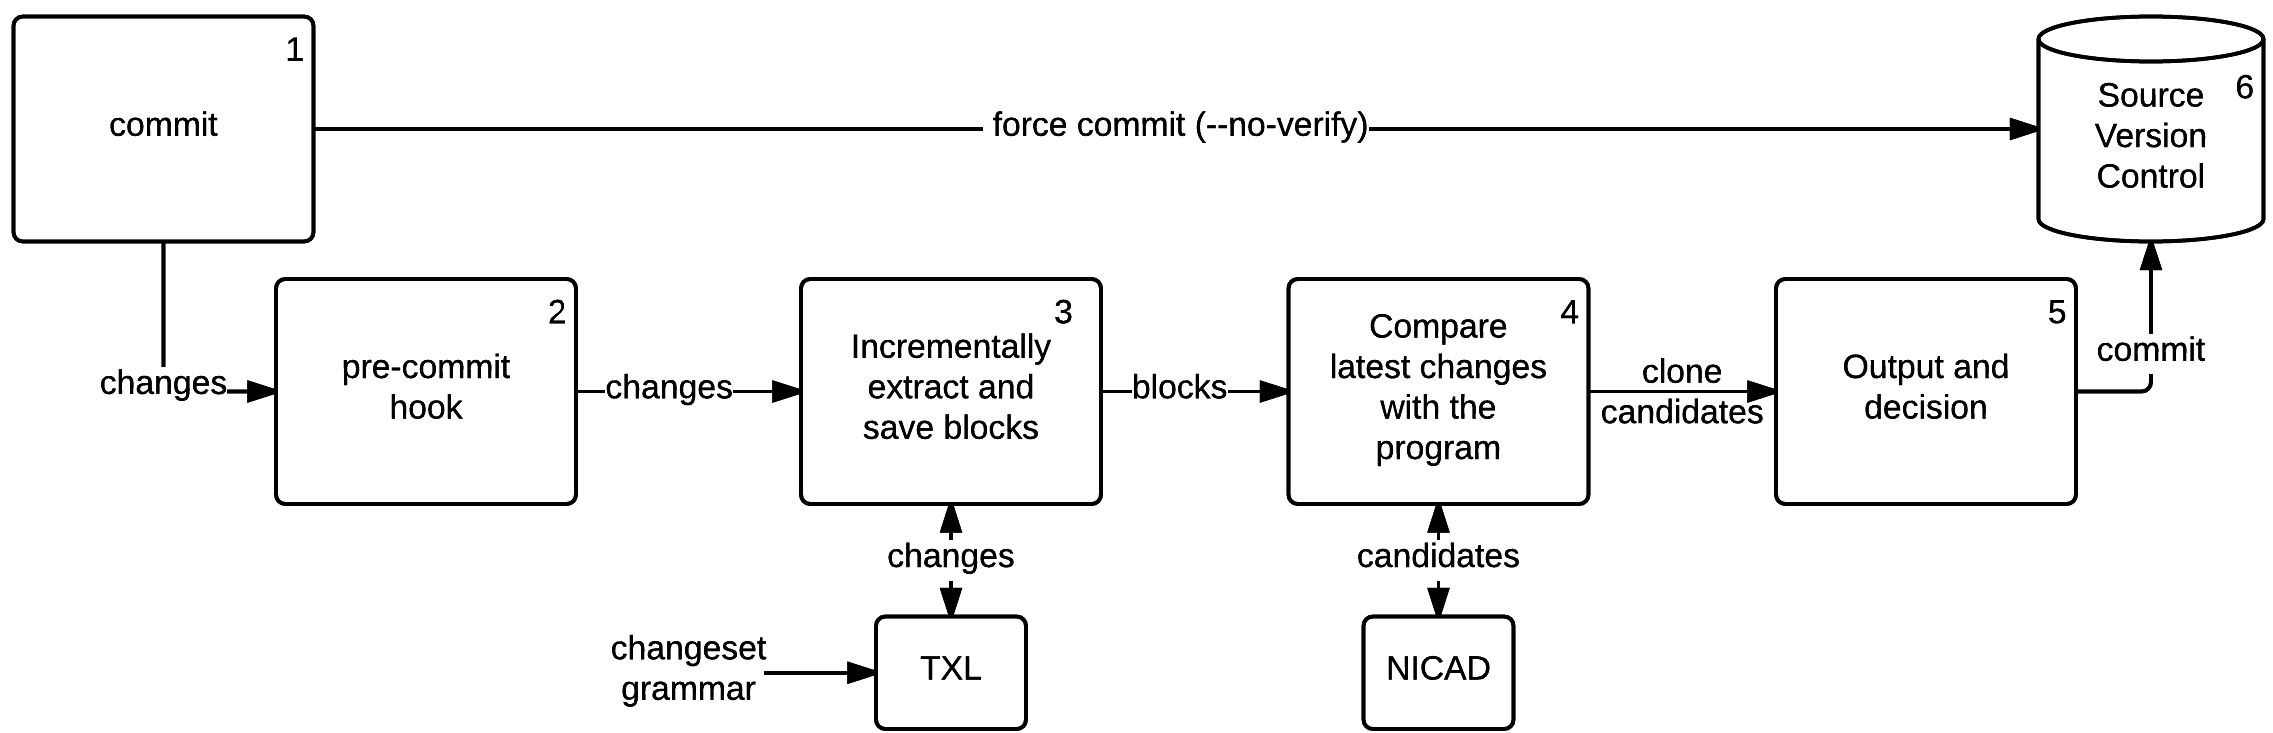
\includegraphics[width=\textwidth]{media/approach.png}
    \caption{ Overview of the PRECINCT Approach.\label{fig:precinct-approach}}
\end{figure*}

\section{Experimentations}
\label{sec:Experimentations}

\section{Conclusion}
\label{sec:Conclusion}







\bibliographystyle{IEEEtran}
\bibliography{library.bib}


\end{document}
